% !TeX TS-program = xelatex

\documentclass{resume}
\ResumeName{\songti  刘华强}
% 如果想插入照片，请使用以下两个库。
\usepackage{graphicx}
\usepackage{tikz}
\usepackage{enumitem}
\usepackage{xcolor}
\definecolor{myblue}{RGB}{0,48,96}
\definecolor{deepred}{RGB}{120,20,20}
% \definecolor{myblue}{RGB}{0,0,0}
% \definecolor{deepred}{RGB}{0,0,0}

\begin{document}

\begin{tikzpicture}[remember picture, overlay]
  \node[anchor=north east] at ([xshift=-0.6cm,yshift=-1.15cm]current page.north east) {
    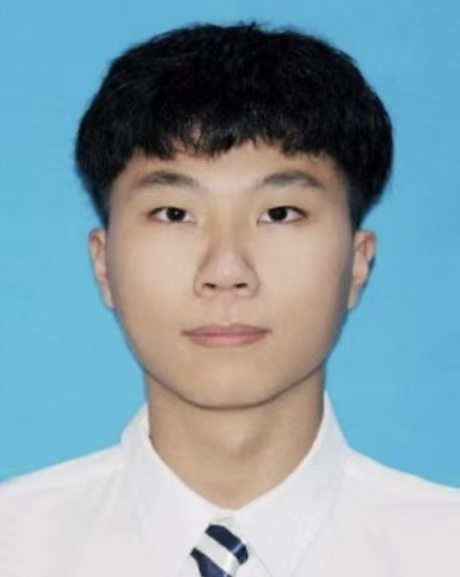
\includegraphics[width=2.4cm,height=3.2cm]{photo}
  };
\end{tikzpicture}
\small
\begin{flushleft}


\ResumeContacts{\zihao{5}
  15045468496,%
  liuhq317@163.com,%
  huaqliu.github.io
}

\ResumeTitle

% Balance the header spacing while keeping the resume on one page.
\vspace{-0.2em}



\textbf{{求职意向：}}运动控制算法实习生\\
\textbf{到岗安排：}随时到岗，每周到岗5天，可实习6个月以上。\\

\textbf{哈尔滨工业大学}
[\textnormal{航天学院｜自动化｜工学学士 2022.08—2026.06}]\\

\textbf{哈尔滨工业大学}
[\textnormal{航天学院｜控制科学与工程｜工学硕士 2026.09—2029.06}]


\textbf{本科学分绩：92.268}，\textbf{综合排名：9/108}，\textbf{国家奖学金、人民奖学金等累计奖学金2w+}

\end{flushleft}


\section{\textcolor{myblue}{实习经历}}

\ResumeItem{\textbf{将闲科技（LiberAI）}}
[\textcolor{deepred}{\ 机器人运动控制实习生}]
[2026.05—2026.09]

\begin{itemize}
  \item \textbf{运控系统与动作部署：}负责\textbf{开发在线负载辨识系统}，参与\textbf{运动控制系统设计}与\textbf{双臂遥操作系统维护}，协同模型组开展上层模型的真机部署与联调，处理控制器参数、动作缓冲区、插值与滤波等问题，确保遥操作与模型输出动作的安全、精确执行。
  \item \textbf{底盘控制与真机联调：}完成 \textbf{Tidybot 8电机舵轮底盘正逆运动学解算、处理零力矩点}及\textbf{真机部署}，开展底层硬件与上层控制模块的联合调试，并将功能封装为\textbf{SDK}便于调用。
  \item \textbf{机器人建模与参数校正：}负责 Leo 机器人\textbf{URDF/MJCF }模型构建与校正，完成连杆质量与惯性参数、关节坐标系、碰撞几何等模型配置及调试，支撑机器人运动学、动力学与碰撞仿真验证。
  \item[] \textit{\textcolor{deepred}{技术栈：}运动控制、在线负载辨识、底盘运动学、双臂遥操作、URDF/MJCF、MuJoCo、SDK封装。}
\end{itemize}

\section{\textcolor{myblue}{项目经历}}

\ResumeItem{\textbf{机械臂在线负载辨识与动力学估计}}
[\textcolor{deepred}{\ LiberAI开发项目}]
[2026.05—2026.09]

\begin{itemize}
  \item[] \textbf{项目背景：}模型输出的 \textbf{Action Chunks} 为相对运动量，当模型控制机械臂时，由于末端未知负载并未被重力补偿，机械臂会持续缓慢下垂。项目旨在通过\textbf{在线负载辨识}，为负载补偿提供参数依据。
  \item \textbf{论文调研与方案选型：}检索并梳理机械臂动力学参数辨识与在线负载估计相关论文，对比 \textbf{RLS 与 MHE} 的建模假设、实时性及噪声鲁棒性，为在线辨识方案选型提供依据。
  \item \textbf{在线负载估计：}开发基于\textbf{机器人动力学回归模型}、\textbf{凸优化理论}、\textbf{递推最小二乘（RLS）}与\textbf{滚动时域估计（MHE）}的在线负载辨识系统，无需运行专用辨识轨迹，利用任务执行中的反馈数据在后台实时估计末端负载。
  \item \textbf{动力学参数辨识：}设计\textbf{摩擦力辨识与机械臂动力学参数辨识}方案，为在线负载估计提供模型基础，降低模型误差对辨识精度的影响。
  \item \textbf{SDK封装与接口设计：}将负载辨识算法封装为\textbf{可复用模块}，提供\textbf{状态输入与估计结果输出接口}，支持运控系统集成调用。
  \item[] \textit{\textcolor{deepred}{技术栈：}动力学回归、RLS、MHE、摩擦辨识、在线参数估计、SDK封装。}
\end{itemize}

\ResumeItem{\textbf{基于视觉-语言大模型的机械臂智能抓取研究}}
[\textcolor{deepred}{\ 本科毕业设计}]
[2025.06—2026.04]

\begin{itemize}
  \item \textbf{系统搭建与任务流程：}基于 \textbf{Ubuntu、ROS2} 搭建 \textbf{Franka 七自由度机械臂}抓取系统，设计自然语言指令驱动的抓取流程，完成感知、规划与控制模块的集成与真机联调。
  \item \textbf{运动规划与控制：}设计并应用\textbf{关节空间与笛卡尔空间阻抗控制、力位混合控制等}，完成目标抓取位姿到机械臂动作执行的控制流程。
  \item \textbf{感知与抓取闭环：}集成 \textbf{Qwen3-VL、SAM、GraspNet}，实现指令理解、目标识别与定位、图像分割及抓取位姿生成，并对接机械臂控制模块，形成\textbf{自然语言指令到真机抓取执行}的完整闭环。
  \item[] \textit{\textcolor{deepred}{技术栈：}ROS2、Franka、阻抗控制、VLM、SAM、GraspNet。}
\end{itemize}

\section{\textcolor{myblue}{竞赛经历}}

\ResumeItem{\textbf{RoboMaster 全国大学生机器人大赛}}
[\textcolor{deepred}{\ 全国一等奖｜空中机器人组负责人}]
[2023.08—2025.08][\small]

\begin{itemize}
  \item \textbf{研发统筹：}负责全赛季无人机系统研发与制作，协调\textbf{机械、电控与视觉}模块协同开发，推进系统集成与整机联调。
  \item \textbf{飞控与定位：}完成无人机飞控设计与参数调试，结合\textbf{激光雷达} 实现定位。
  \item \textbf{云台控制：}负责三轴云台\textbf{PID 调参与视觉伺服}，实现对高速移动目标的稳定跟踪。
\end{itemize}

\ResumeItem{\textbf{中国大学生工程实践与创新能力大赛}}
[\textcolor{deepred}{\ 全国一等奖｜队长}]
[2025.01—2025.08][\small]

\begin{itemize}
  \item \textbf{电控与协同控制：}负责系统电控方案及整机控制逻辑设计，实现\textbf{SCARA 机械臂与麦轮底盘协同控制}。
  \item \textbf{任务执行：}独立设计\textbf{整机状态机与多阶段动作调度}，集成视觉伺服与抓取控制，完成自动搬运及软硬件联调。
\end{itemize}

\ResumeItem{\textbf{全国大学生电子设计竞赛—无人机赛题}}
[\textcolor{deepred}{\ 全国二等奖｜队长}]
[2024.05—2025.08][\small]

\begin{itemize}
  \item \textbf{系统开发：}完成四旋翼无人机方案设计、硬件集成、控制算法开发及任务流程设计，负责整机调试。
  \item \textbf{飞控与视觉：}负责\textbf{多层 PID 参数整定与视觉伺服}，结合视觉识别实现目标搜索与跟踪，优化飞行稳定性与执行精度。
\end{itemize}

\section{\textcolor{myblue}{技术能力}}
\begin{itemize}
  \item \textbf{机器人建模与动力学}: 熟悉机械臂\textbf{正逆运动学、雅可比矩阵及刚体动力学}，具备 \textbf{URDF / MJCF} 模型构建与校正、\textbf{动力学回归建模及 RLS 在线参数辨识}经验，有丰富的真实机器人设计与调试的经验。
  \item \textbf{运动控制与真机调试}: 具备 \textbf{关节空间 / 笛卡尔空间阻抗控制、轨迹规划、插值与滤波}经验，熟悉多层 PID 控制及参数整定，具有机器人控制器调试与真机动作部署经验。
  \item \textbf{编程与工程开发}: 熟悉 \textbf{C/C++、Python}，具备机器人控制算法开发、\textbf{SDK 接口封装、软硬件联调}及机器人系统工程化实现经验。
  \item \textbf{机器人平台与仿真}: 熟悉 \textbf{Ubuntu、ROS2、MoveIt2、MuJoCo}，具备 \textbf{Franka 机械臂、移动底盘}的建模、仿真及控制开发经验，了解 STM32、FreeRTOS 嵌入式开发。
\end{itemize}

\end{document}
